\documentclass[tikz,border=5pt]{standalone}
\usepackage{amsmath,amssymb}
\usepackage{tikz}
\usetikzlibrary{arrows.meta,positioning,fit,calc,shapes.geometric,shapes.misc}
\usepackage{tcolorbox}

% Canonical MLSys Book Volume 1 & Volume 3 Color Palette
\definecolor{DarkSlate}{HTML}{0F172A}
\definecolor{slatesteel}{HTML}{475569}
\definecolor{coolparchment}{HTML}{F8FAFC}
\definecolor{GridGray}{HTML}{E2E8F0}

\definecolor{BlueLine}{HTML}{0284C7}
\definecolor{BlueL0}{HTML}{F0F9FF}
\definecolor{deepcyan}{HTML}{0369A1}

\definecolor{GreenLine}{HTML}{16A34A}
\definecolor{GreenL0}{HTML}{F0FDF4}
\definecolor{forestsage}{HTML}{15803D}

\definecolor{OrangeLine}{HTML}{EA580C}
\definecolor{OrangeL0}{HTML}{FFFBEB}
\definecolor{warmochre}{HTML}{B45309}

\definecolor{RedLine}{HTML}{DC2626}
\definecolor{RedL0}{HTML}{FEF2F2}
\definecolor{deepburgundy}{HTML}{991B1B}

\definecolor{PurpleLine}{HTML}{7C3AED}
\definecolor{PurpleL0}{HTML}{FAF5FF}
\definecolor{deeproyal}{HTML}{5B21B6}

\begin{document}
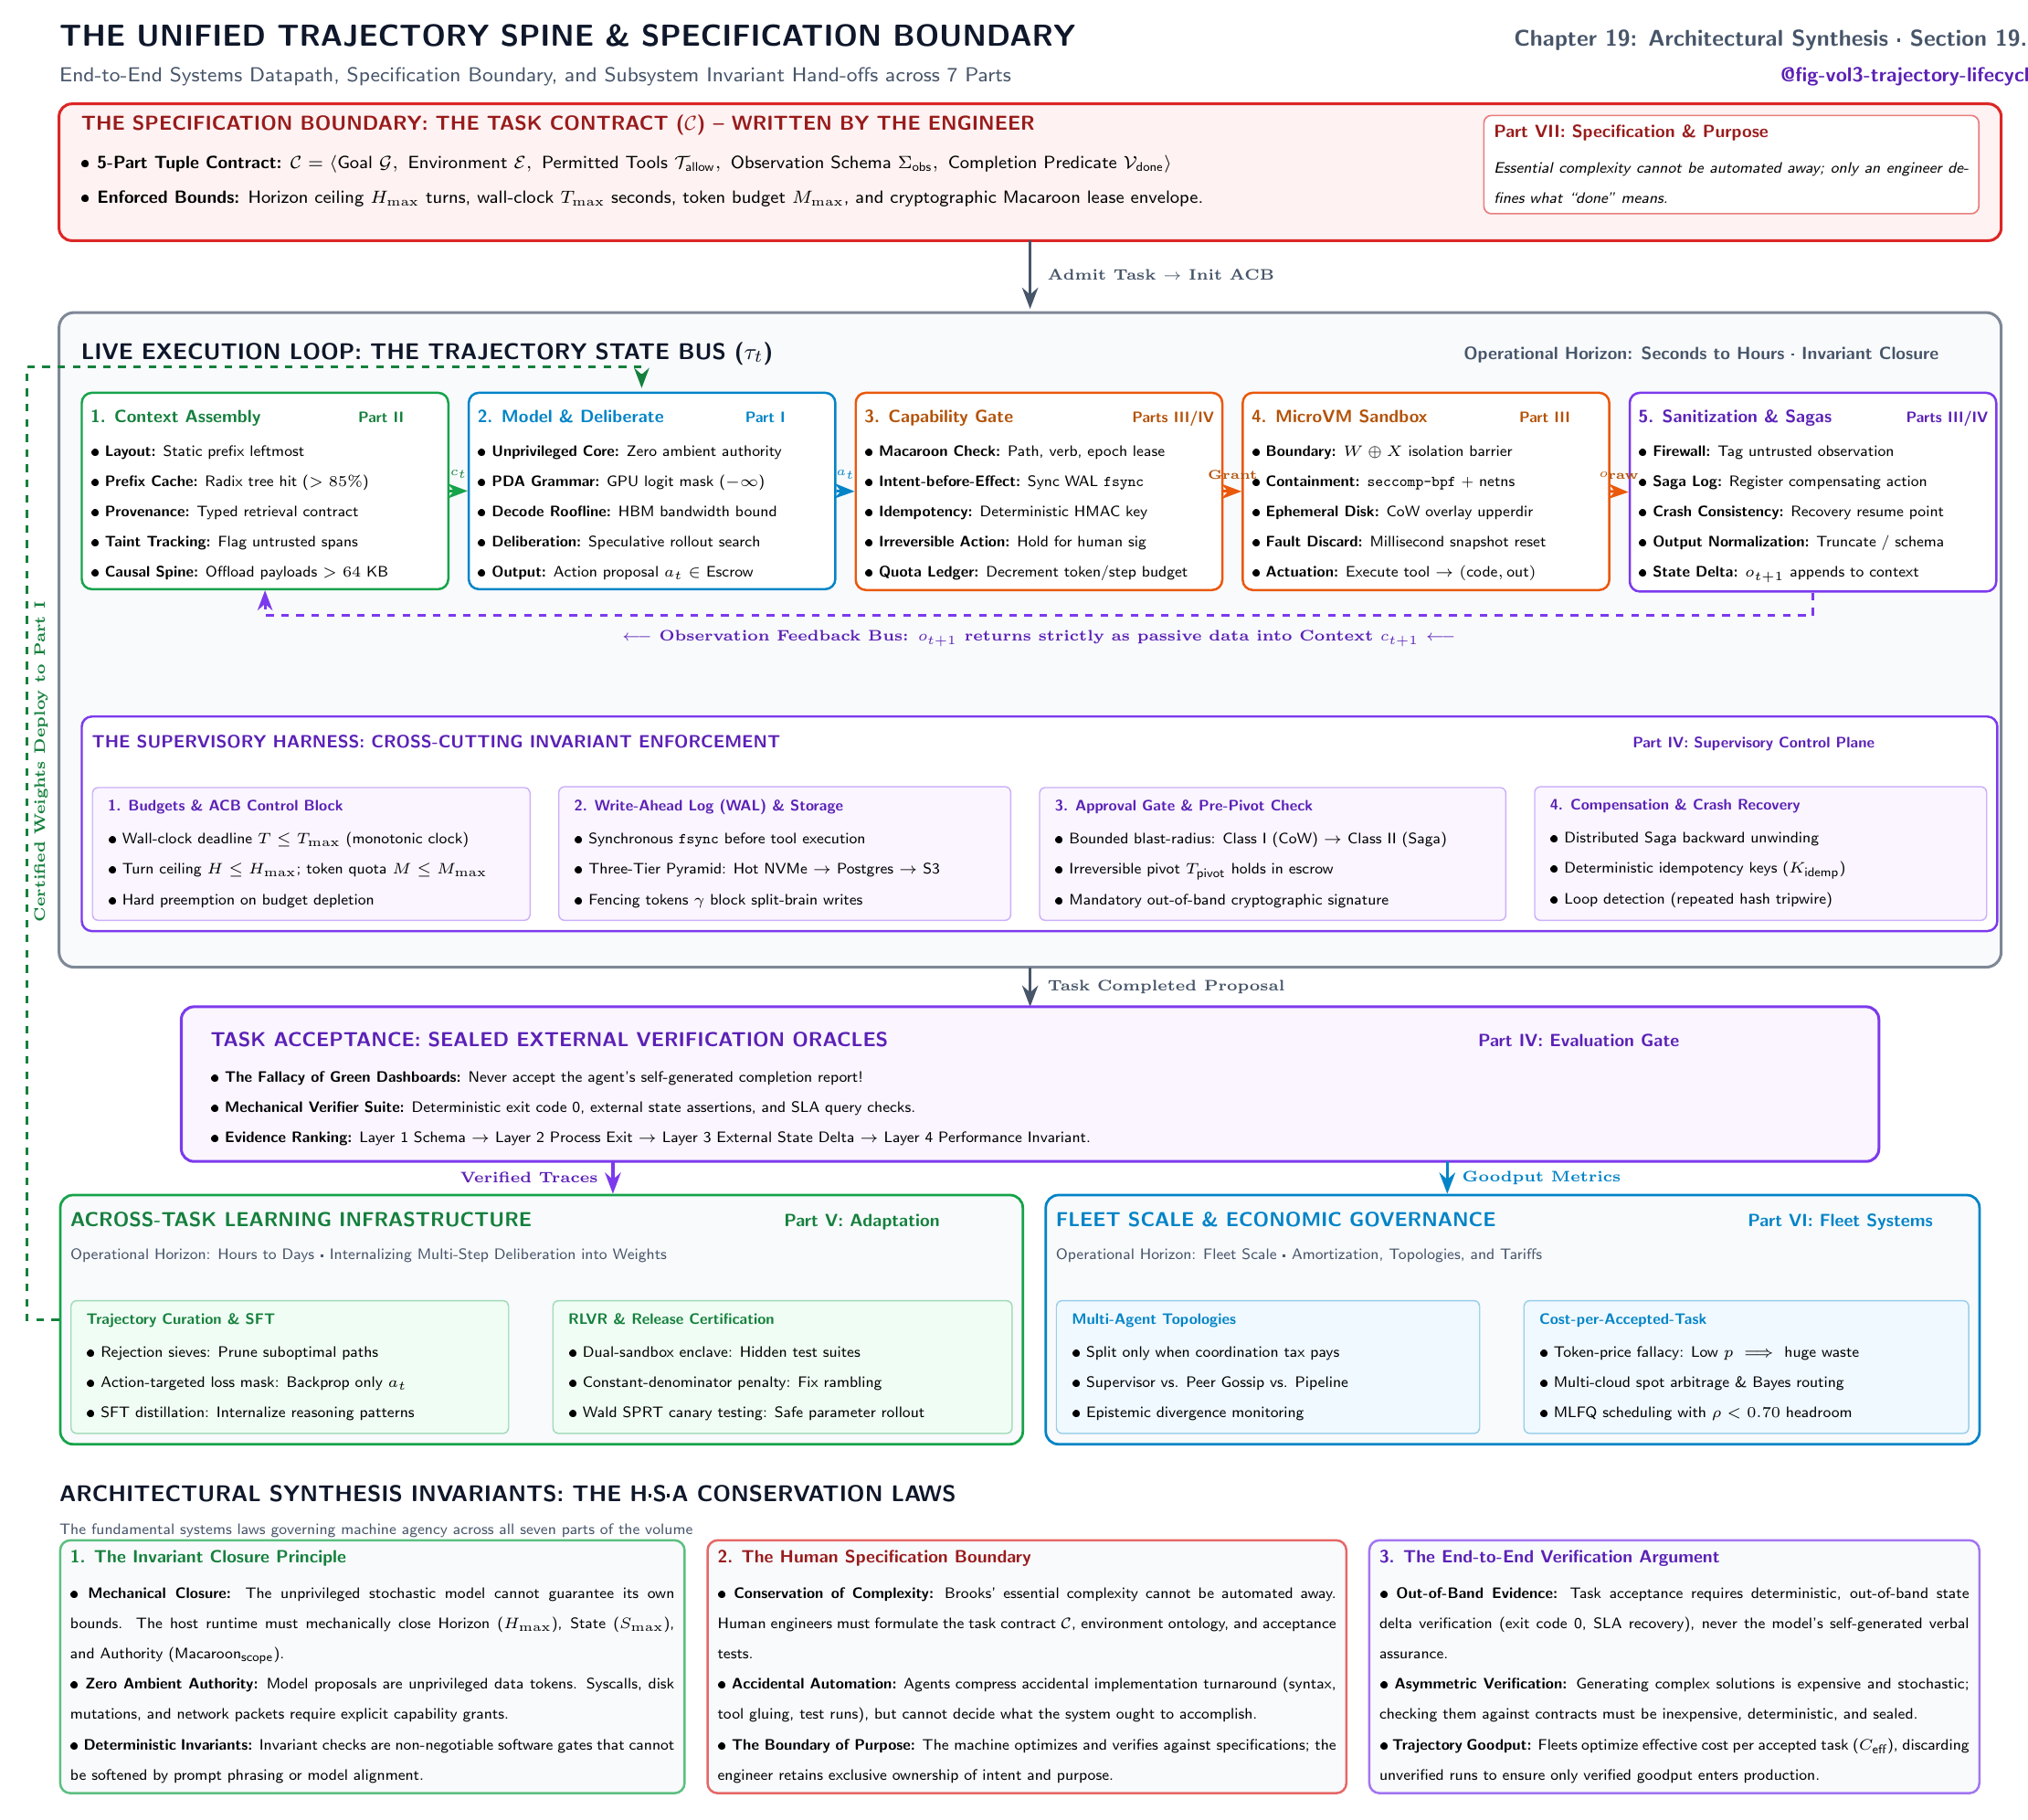
\begin{tikzpicture}[
  font=\sffamily,
  scale=1.0,
  >=Stealth,
  node distance=0.5cm
]

% =============================================================
% MASTER TITLE BANNER
% =============================================================
\node[anchor=north west, inner sep=0pt] (title) at (0.8, 25.4) {
  \begin{minipage}{27.0cm}
    \begin{tabular}{@{}p{19.8cm} r@{}}
      {\fontsize{12}{15}\selectfont \textbf{\textcolor{DarkSlate}{THE UNIFIED TRAJECTORY SPINE \& SPECIFICATION BOUNDARY}}} &
      \fontsize{9}{11.5}\selectfont \textcolor{slatesteel}{\textbf{Chapter 19: Architectural Synthesis · Section 19.2}} \\[2pt]
      {\fontsize{8.5}{11}\selectfont \textcolor{slatesteel}{End-to-End Systems Datapath, Specification Boundary, and Subsystem Invariant Hand-offs across 7 Parts}} &
      \fontsize{8}{10}\selectfont \textcolor{deeproyal}{\textbf{@fig-vol3-trajectory-lifecycle}} \\
    \end{tabular}
  \end{minipage}
};

% =============================================================
% LEVEL 0: THE SPECIFICATION BOUNDARY (PART VII)
% =============================================================
\draw[draw=RedLine, fill=RedL0, line width=1.1pt, rounded corners=5pt] 
  (0.8, 24.3) rectangle (27.8, 22.4);

% Left content: Contract and bounds
\node[anchor=north west, inner sep=0pt] at (1.1, 24.15) {
  \begin{minipage}{19.2cm}
    {\fontsize{8.5}{10.5}\selectfont \textbf{\textcolor{deepburgundy}{THE SPECIFICATION BOUNDARY: THE TASK CONTRACT ($\mathcal{C}$) -- WRITTEN BY THE ENGINEER}}}\\[3pt]
    {\fontsize{6.8}{8.2}\selectfont
    \textbullet\ \textbf{5-Part Tuple Contract:} $\mathcal{C} = \langle \text{Goal } \mathcal{G}, \text{ Environment } \mathcal{E}, \text{ Permitted Tools } \mathcal{T}_{\text{allow}}, \text{ Observation Schema } \Sigma_{\text{obs}}, \text{ Completion Predicate } \mathcal{V}_{\text{done}} \rangle$\\[2pt]
    \textbullet\ \textbf{Enforced Bounds:} Horizon ceiling $H_{\max}$ turns, wall-clock $T_{\max}$ seconds, token budget $M_{\max}$, and cryptographic Macaroon lease envelope.
    }
  \end{minipage}
};

% Right callout card: Part VII badge
\node[anchor=north east, fill=white, draw=RedLine!60, line width=0.6pt, rounded corners=3pt, inner sep=4pt] 
  at (27.5, 24.15) {
  \begin{minipage}{6.6cm}
    {\fontsize{6.8}{8.2}\selectfont \textbf{\textcolor{deepburgundy}{Part VII: Specification \& Purpose}}}\\[2pt]
    {\fontsize{5.8}{7}\selectfont \textit{Essential complexity cannot be automated away; only an engineer defines what ``done'' means.}}
  \end{minipage}
};

% Downward arrow to Live Loop
\draw[->, draw=slatesteel, line width=1.2pt] (14.3, 22.4) -- (14.3, 21.45) 
  node[midway, right=3pt, font=\fontsize{6.2}{7.5}\selectfont\bfseries, text=slatesteel] {Admit Task $\to$ Init ACB};

% =============================================================
% LEVEL 1: THE LIVE EXECUTION LOOP (ONE TRAJECTORY: SECONDS TO HOURS)
% =============================================================
\draw[draw=slatesteel!70, fill=coolparchment, line width=1.1pt, rounded corners=6pt] 
  (0.8, 21.4) rectangle (27.8, 12.3);

% Header Band
\node[anchor=north west, inner sep=0pt] at (1.1, 21.05) {
  \begin{minipage}{26.4cm}
    \begin{tabular}{@{}p{18.8cm} r@{}}
      {\fontsize{9.5}{11.5}\selectfont \textbf{\textcolor{DarkSlate}{LIVE EXECUTION LOOP: THE TRAJECTORY STATE BUS ($\tau_t$)}}} &
      \fontsize{7.5}{9.5}\selectfont \textcolor{slatesteel}{\textbf{Operational Horizon: Seconds to Hours · Invariant Closure}}
    \end{tabular}
  \end{minipage}
};

% -------------------------------------------------------------
% FIVE SEQUENTIAL CORE DATAPATH STAGES
% -------------------------------------------------------------

% Stage 1: Context Assembly (Part II)
\node[anchor=north west, fill=white, draw=GreenLine, line width=0.9pt, rounded corners=4pt, inner sep=3.5pt] 
  (s1_context) at (1.1, 20.3) {
  \begin{minipage}{4.85cm}
    \begin{tabular}{@{}p{3.3cm} r@{}}
      {\fontsize{7.2}{8.5}\selectfont \textbf{\textcolor{forestsage}{1. Context Assembly}}} &
      \fontsize{6.2}{7.5}\selectfont \textbf{\textcolor{forestsage}{Part II}}
    \end{tabular}\\[1pt]
    {\fontsize{5.8}{7}\selectfont
    \textbullet\ \textbf{Layout:} Static prefix leftmost\\
    \textbullet\ \textbf{Prefix Cache:} Radix tree hit ($>85\%$)\\
    \textbullet\ \textbf{Provenance:} Typed retrieval contract\\
    \textbullet\ \textbf{Taint Tracking:} Flag untrusted spans\\
    \textbullet\ \textbf{Causal Spine:} Offload payloads $>64\text{ KB}$
    }
  \end{minipage}
};

% Stage 2: Inference & Deliberation (Part I)
\node[anchor=north west, fill=white, draw=BlueLine, line width=0.9pt, rounded corners=4pt, inner sep=3.5pt] 
  (s2_model) at (6.48, 20.3) {
  \begin{minipage}{4.85cm}
    \begin{tabular}{@{}p{3.3cm} r@{}}
      {\fontsize{7.2}{8.5}\selectfont \textbf{\textcolor{BlueLine}{2. Model \& Deliberate}}} &
      \fontsize{6.2}{7.5}\selectfont \textbf{\textcolor{BlueLine}{Part I}}
    \end{tabular}\\[1pt]
    {\fontsize{5.8}{7}\selectfont
    \textbullet\ \textbf{Unprivileged Core:} Zero ambient authority\\
    \textbullet\ \textbf{PDA Grammar:} GPU logit mask ($-\infty$)\\
    \textbullet\ \textbf{Decode Roofline:} HBM bandwidth bound\\
    \textbullet\ \textbf{Deliberation:} Speculative rollout search\\
    \textbullet\ \textbf{Output:} Action proposal $a_t \in \text{Escrow}$
    }
  \end{minipage}
};

% Stage 3: Capability Gate & Policy (Part III & IV)
\node[anchor=north west, fill=white, draw=OrangeLine, line width=0.9pt, rounded corners=4pt, inner sep=3.5pt] 
  (s3_gate) at (11.86, 20.3) {
  \begin{minipage}{4.85cm}
    \begin{tabular}{@{}p{3.3cm} r@{}}
      {\fontsize{7.2}{8.5}\selectfont \textbf{\textcolor{warmochre}{3. Capability Gate}}} &
      \fontsize{6.2}{7.5}\selectfont \textbf{\textcolor{warmochre}{Parts III/IV}}
    \end{tabular}\\[1pt]
    {\fontsize{5.8}{7}\selectfont
    \textbullet\ \textbf{Macaroon Check:} Path, verb, epoch lease\\
    \textbullet\ \textbf{Intent-before-Effect:} Sync WAL \texttt{fsync}\\
    \textbullet\ \textbf{Idempotency:} Deterministic HMAC key\\
    \textbullet\ \textbf{Irreversible Action:} Hold for human sig\\
    \textbullet\ \textbf{Quota Ledger:} Decrement token/step budget
    }
  \end{minipage}
};

% Stage 4: MicroVM Sandbox (Part III)
\node[anchor=north west, fill=white, draw=OrangeLine, line width=0.9pt, rounded corners=4pt, inner sep=3.5pt] 
  (s4_sandbox) at (17.24, 20.3) {
  \begin{minipage}{4.85cm}
    \begin{tabular}{@{}p{3.3cm} r@{}}
      {\fontsize{7.2}{8.5}\selectfont \textbf{\textcolor{warmochre}{4. MicroVM Sandbox}}} &
      \fontsize{6.2}{7.5}\selectfont \textbf{\textcolor{warmochre}{Part III}}
    \end{tabular}\\[1pt]
    {\fontsize{5.8}{7}\selectfont
    \textbullet\ \textbf{Boundary:} $W \oplus X$ isolation barrier\\
    \textbullet\ \textbf{Containment:} \texttt{seccomp-bpf} + netns\\
    \textbullet\ \textbf{Ephemeral Disk:} CoW overlay upperdir\\
    \textbullet\ \textbf{Fault Discard:} Millisecond snapshot reset\\
    \textbullet\ \textbf{Actuation:} Execute tool $\to (\text{code}, \text{out})$
    }
  \end{minipage}
};

% Stage 5: Observation Sanitization & Sagas (Part III & IV)
\node[anchor=north west, fill=white, draw=PurpleLine, line width=0.9pt, rounded corners=4pt, inner sep=3.5pt] 
  (s5_obs) at (22.62, 20.3) {
  \begin{minipage}{4.85cm}
    \begin{tabular}{@{}p{3.3cm} r@{}}
      {\fontsize{7.2}{8.5}\selectfont \textbf{\textcolor{deeproyal}{5. Sanitization \& Sagas}}} &
      \fontsize{6.2}{7.5}\selectfont \textbf{\textcolor{deeproyal}{Parts III/IV}}
    \end{tabular}\\[1pt]
    {\fontsize{5.8}{7}\selectfont
    \textbullet\ \textbf{Firewall:} Tag untrusted observation\\
    \textbullet\ \textbf{Saga Log:} Register compensating action\\
    \textbullet\ \textbf{Crash Consistency:} Recovery resume point\\
    \textbullet\ \textbf{Output Normalization:} Truncate / schema\\
    \textbullet\ \textbf{State Delta:} $o_{t+1}$ appends to context
    }
  \end{minipage}
};

% Forward Datapath Arrows with compact labels
\draw[->, draw=GreenLine, line width=1.1pt] (s1_context.east) -- (s2_model.west)
  node[midway, above=1pt, font=\fontsize{5.4}{6.8}\selectfont\bfseries, text=forestsage] {$c_t$};

\draw[->, draw=BlueLine, line width=1.1pt] (s2_model.east) -- (s3_gate.west)
  node[midway, above=1pt, font=\fontsize{5.4}{6.8}\selectfont\bfseries, text=BlueLine] {$a_t$};

\draw[->, draw=OrangeLine, line width=1.1pt] (s3_gate.east) -- (s4_sandbox.west)
  node[midway, above=1pt, font=\fontsize{5.4}{6.8}\selectfont\bfseries, text=warmochre] {Grant};

\draw[->, draw=OrangeLine, line width=1.1pt] (s4_sandbox.east) -- (s5_obs.west)
  node[midway, above=1pt, font=\fontsize{5.4}{6.8}\selectfont\bfseries, text=warmochre] {$o_{\text{raw}}$};

% Observation Feedback Bus (Dashed)
\draw[->, draw=PurpleLine, line width=1.1pt, dashed] 
  (s5_obs.south) -- ++(0, -0.32) -| (s1_context.south)
  node[pos=0.25, below=2pt, font=\fontsize{6.2}{7.5}\selectfont\bfseries, text=deeproyal] 
  {$\longleftarrow$ Observation Feedback Bus: $o_{t+1}$ returns strictly as passive data into Context $c_{t+1}$ $\longleftarrow$};

% -------------------------------------------------------------
% SUB-LAYER: THE SUPERVISORY HARNESS (PART IV)
% -------------------------------------------------------------
\node[anchor=north west, fill=white, draw=PurpleLine, line width=0.9pt, rounded corners=4pt, inner sep=4pt] 
  (harness_band) at (1.1, 15.8) {
  \begin{minipage}{26.35cm}
    \begin{tabular}{@{}p{21.0cm} r@{}}
      {\fontsize{7.5}{9}\selectfont \textbf{\textcolor{deeproyal}{THE SUPERVISORY HARNESS: CROSS-CUTTING INVARIANT ENFORCEMENT}}} &
      \fontsize{6.5}{8}\selectfont \textcolor{deeproyal}{\textbf{Part IV: Supervisory Control Plane}}
    \end{tabular}\\[2pt]
    
    % Four sub-cards inside the harness
    \begin{minipage}[t]{6.1cm}
      \begin{tcolorbox}[colback=PurpleL0, colframe=PurpleLine!40, arc=2pt, boxrule=0.5pt, left=3pt, right=3pt, top=2pt, bottom=2pt]
        {\fontsize{6.5}{7.5}\selectfont \textbf{\textcolor{deeproyal}{1. Budgets \& ACB Control Block}}}\\[1pt]
        {\fontsize{5.6}{6.8}\selectfont
        \textbullet\ Wall-clock deadline $T \le T_{\max}$ (monotonic clock)\\
        \textbullet\ Turn ceiling $H \le H_{\max}$; token quota $M \le M_{\max}$\\
        \textbullet\ Hard preemption on budget depletion
        }
      \end{tcolorbox}
    \end{minipage}\hfill
    \begin{minipage}[t]{6.3cm}
      \begin{tcolorbox}[colback=PurpleL0, colframe=PurpleLine!40, arc=2pt, boxrule=0.5pt, left=3pt, right=3pt, top=2pt, bottom=2pt]
        {\fontsize{6.5}{7.5}\selectfont \textbf{\textcolor{deeproyal}{2. Write-Ahead Log (WAL) \& Storage}}}\\[1pt]
        {\fontsize{5.6}{6.8}\selectfont
        \textbullet\ Synchronous \texttt{fsync} before tool execution\\
        \textbullet\ Three-Tier Pyramid: Hot NVMe $\to$ Postgres $\to$ S3\\
        \textbullet\ Fencing tokens $\gamma$ block split-brain writes
        }
      \end{tcolorbox}
    \end{minipage}\hfill
    \begin{minipage}[t]{6.5cm}
      \begin{tcolorbox}[colback=PurpleL0, colframe=PurpleLine!40, arc=2pt, boxrule=0.5pt, left=3pt, right=3pt, top=2pt, bottom=2pt]
        {\fontsize{6.5}{7.5}\selectfont \textbf{\textcolor{deeproyal}{3. Approval Gate \& Pre-Pivot Check}}}\\[1pt]
        {\fontsize{5.6}{6.8}\selectfont
        \textbullet\ Bounded blast-radius: Class I (CoW) $\to$ Class II (Saga)\\
        \textbullet\ Irreversible pivot $T_{\text{pivot}}$ holds in escrow\\
        \textbullet\ Mandatory out-of-band cryptographic signature
        }
      \end{tcolorbox}
    \end{minipage}\hfill
    \begin{minipage}[t]{6.3cm}
      \begin{tcolorbox}[colback=PurpleL0, colframe=PurpleLine!40, arc=2pt, boxrule=0.5pt, left=3pt, right=3pt, top=2pt, bottom=2pt]
        {\fontsize{6.5}{7.5}\selectfont \textbf{\textcolor{deeproyal}{4. Compensation \& Crash Recovery}}}\\[1pt]
        {\fontsize{5.6}{6.8}\selectfont
        \textbullet\ Distributed Saga backward unwinding\\
        \textbullet\ Deterministic idempotency keys ($K_{\text{idemp}}$)\\
        \textbullet\ Loop detection (repeated hash tripwire)
        }
      \end{tcolorbox}
    \end{minipage}
  \end{minipage}
};

% Downward arrow to Acceptance
\draw[->, draw=slatesteel, line width=1.2pt] (14.3, 12.3) -- (14.3, 11.75) 
  node[midway, right=3pt, font=\fontsize{6.2}{7.5}\selectfont\bfseries, text=slatesteel] {Task Completed Proposal};

% =============================================================
% LEVEL 2: SEALED ACCEPTANCE GATE (PART IV & VII)
% =============================================================
\draw[draw=PurpleLine, fill=PurpleL0, line width=1.1pt, rounded corners=5pt] 
  (2.5, 11.75) rectangle (26.1, 9.6);

\node[anchor=north west, inner sep=0pt] at (2.9, 11.5) {
  \begin{minipage}{22.8cm}
    \begin{tabular}{@{}p{17.2cm} r@{}}
      {\fontsize{8.5}{10.5}\selectfont \textbf{\textcolor{deeproyal}{TASK ACCEPTANCE: SEALED EXTERNAL VERIFICATION ORACLES}}} &
      \fontsize{6.8}{8.2}\selectfont \textbf{\textcolor{deeproyal}{Part IV: Evaluation Gate}}
    \end{tabular}\\[2pt]
    {\fontsize{6.3}{7.8}\selectfont
    \textbullet\ \textbf{The Fallacy of Green Dashboards:} Never accept the agent's self-generated completion report!\\
    \textbullet\ \textbf{Mechanical Verifier Suite:} Deterministic exit code 0, external state assertions, and SLA query checks.\\
    \textbullet\ \textbf{Evidence Ranking:} Layer 1 Schema $\to$ Layer 2 Process Exit $\to$ Layer 3 External State Delta $\to$ Layer 4 Performance Invariant.
    }
  \end{minipage}
};

% Downward bifurcated arrows to Across-Task Horizons
\draw[->, draw=PurpleLine, line width=1.2pt] (8.5, 9.6) -- (8.5, 9.15)
  node[midway, left=2pt, font=\fontsize{6.0}{7.2}\selectfont\bfseries, text=deeproyal] {Verified Traces};

\draw[->, draw=BlueLine, line width=1.2pt] (20.1, 9.6) -- (20.1, 9.15)
  node[midway, right=2pt, font=\fontsize{6.0}{7.2}\selectfont\bfseries, text=BlueLine] {Goodput Metrics};

% =============================================================
% LEVEL 3: ACROSS-TASK LIFECYCLE INFRASTRUCTURE (HOURS TO DAYS)
% =============================================================

% Left Card: Across-Task Learning (Part V)
\node[anchor=north west, fill=coolparchment, draw=GreenLine, line width=1.0pt, rounded corners=5pt, inner sep=4pt] 
  (c_learning) at (0.8, 9.15) {
  \begin{minipage}{13.1cm}
    \begin{tabular}{@{}p{9.5cm} r@{}}
      {\fontsize{8.5}{10.5}\selectfont \textbf{\textcolor{forestsage}{ACROSS-TASK LEARNING INFRASTRUCTURE}}} &
      \fontsize{6.8}{8.2}\selectfont \textbf{\textcolor{forestsage}{Part V: Adaptation}}
    \end{tabular}\\[1pt]
    {\fontsize{6.0}{7.2}\selectfont \textcolor{slatesteel}{Operational Horizon: Hours to Days · Internalizing Multi-Step Deliberation into Weights}}\\[3pt]
    
    \begin{minipage}[t]{6.1cm}
      \begin{tcolorbox}[colback=GreenL0, colframe=GreenLine!40, arc=2pt, boxrule=0.5pt, left=3pt, right=3pt, top=2pt, bottom=2pt]
        {\fontsize{6.5}{7.5}\selectfont \textbf{\textcolor{forestsage}{Trajectory Curation \& SFT}}}\\[1pt]
        {\fontsize{5.6}{6.8}\selectfont
        \textbullet\ Rejection sieves: Prune suboptimal paths\\
        \textbullet\ Action-targeted loss mask: Backprop only $a_t$\\
        \textbullet\ SFT distillation: Internalize reasoning patterns
        }
      \end{tcolorbox}
    \end{minipage}\hfill
    \begin{minipage}[t]{6.4cm}
      \begin{tcolorbox}[colback=GreenL0, colframe=GreenLine!40, arc=2pt, boxrule=0.5pt, left=3pt, right=3pt, top=2pt, bottom=2pt]
        {\fontsize{6.5}{7.5}\selectfont \textbf{\textcolor{forestsage}{RLVR \& Release Certification}}}\\[1pt]
        {\fontsize{5.6}{6.8}\selectfont
        \textbullet\ Dual-sandbox enclave: Hidden test suites\\
        \textbullet\ Constant-denominator penalty: Fix rambling\\
        \textbullet\ Wald SPRT canary testing: Safe parameter rollout
        }
      \end{tcolorbox}
    \end{minipage}
  \end{minipage}
};

% Feedback from Learning back to Part I (Routes cleanly around Stage 1 through the header corridor)
\draw[->, draw=forestsage, line width=1.1pt, dashed] 
  (c_learning.west) -- ++(-0.45, 0) -- (0.35, 20.65) -- (8.9, 20.65) -- (8.9, 20.35);

\node[anchor=west, font=\fontsize{5.8}{7.0}\selectfont\bfseries, text=forestsage, rotate=90] 
  at (0.55, 12.8) {Certified Weights Deploy to Part I};

% Right Card: Scale & Economics (Part VI)
\node[anchor=north west, fill=coolparchment, draw=BlueLine, line width=1.0pt, rounded corners=5pt, inner sep=4pt] 
  (c_scale) at (14.5, 9.15) {
  \begin{minipage}{12.7cm}
    \begin{tabular}{@{}p{9.2cm} r@{}}
      {\fontsize{8.5}{10.5}\selectfont \textbf{\textcolor{BlueLine}{FLEET SCALE \& ECONOMIC GOVERNANCE}}} &
      \fontsize{6.8}{8.2}\selectfont \textbf{\textcolor{BlueLine}{Part VI: Fleet Systems}}
    \end{tabular}\\[1pt]
    {\fontsize{6.0}{7.2}\selectfont \textcolor{slatesteel}{Operational Horizon: Fleet Scale · Amortization, Topologies, and Tariffs}}\\[3pt]
    
    \begin{minipage}[t]{5.9cm}
      \begin{tcolorbox}[colback=BlueL0, colframe=BlueLine!40, arc=2pt, boxrule=0.5pt, left=3pt, right=3pt, top=2pt, bottom=2pt]
        {\fontsize{6.5}{7.5}\selectfont \textbf{\textcolor{BlueLine}{Multi-Agent Topologies}}}\\[1pt]
        {\fontsize{5.6}{6.8}\selectfont
        \textbullet\ Split only when coordination tax pays\\
        \textbullet\ Supervisor vs. Peer Gossip vs. Pipeline\\
        \textbullet\ Epistemic divergence monitoring
        }
      \end{tcolorbox}
    \end{minipage}\hfill
    \begin{minipage}[t]{6.2cm}
      \begin{tcolorbox}[colback=BlueL0, colframe=BlueLine!40, arc=2pt, boxrule=0.5pt, left=3pt, right=3pt, top=2pt, bottom=2pt]
        {\fontsize{6.5}{7.5}\selectfont \textbf{\textcolor{BlueLine}{Cost-per-Accepted-Task}}}\\[1pt]
        {\fontsize{5.6}{6.8}\selectfont
        \textbullet\ Token-price fallacy: Low $p \implies$ huge waste\\
        \textbullet\ Multi-cloud spot arbitrage \& Bayes routing\\
        \textbullet\ MLFQ scheduling with $\rho < 0.70$ headroom
        }
      \end{tcolorbox}
    \end{minipage}
  \end{minipage}
};

% =============================================================
% LEVEL 4: ARCHITECTURAL SYNTHESIS INVARIANTS & CONSERVATION LAWS
% =============================================================
\node[anchor=north west, inner sep=0pt] at (0.8, 5.1) {
  \begin{minipage}{27.0cm}
    {\fontsize{9.0}{11}\selectfont \textbf{\textcolor{DarkSlate}{ARCHITECTURAL SYNTHESIS INVARIANTS: THE H·S·A CONSERVATION LAWS}}}\\[1pt]
    {\fontsize{6.5}{8}\selectfont \textcolor{slatesteel}{The fundamental systems laws governing machine agency across all seven parts of the volume}}
  \end{minipage}
};

% Three Synthesis Invariant Cards
% Card 1: Invariant Closure
\node[anchor=north west, fill=coolparchment, draw=GreenLine!70, line width=0.9pt, rounded corners=4pt, inner sep=4pt] 
  (inv1) at (0.8, 4.35) {
  \begin{minipage}{8.4cm}
    {\fontsize{7.2}{8.8}\selectfont \textbf{\textcolor{forestsage}{1. The Invariant Closure Principle}}}\\[2pt]
    {\fontsize{5.8}{7}\selectfont
    \textbullet\ \textbf{Mechanical Closure:} The unprivileged stochastic model cannot guarantee its own bounds. The host runtime must mechanically close Horizon ($H_{\max}$), State ($S_{\max}$), and Authority ($\text{Macaroon}_{\text{scope}}$).\\
    \textbullet\ \textbf{Zero Ambient Authority:} Model proposals are unprivileged data tokens. Syscalls, disk mutations, and network packets require explicit capability grants.\\
    \textbullet\ \textbf{Deterministic Invariants:} Invariant checks are non-negotiable software gates that cannot be softened by prompt phrasing or model alignment.
    }
  \end{minipage}
};

% Card 2: The Specification Boundary
\node[anchor=north west, fill=coolparchment, draw=RedLine!70, line width=0.9pt, rounded corners=4pt, inner sep=4pt] 
  (inv2) at (9.8, 4.35) {
  \begin{minipage}{8.6cm}
    {\fontsize{7.2}{8.8}\selectfont \textbf{\textcolor{deepburgundy}{2. The Human Specification Boundary}}}\\[2pt]
    {\fontsize{5.8}{7}\selectfont
    \textbullet\ \textbf{Conservation of Complexity:} Brooks' essential complexity cannot be automated away. Human engineers must formulate the task contract $\mathcal{C}$, environment ontology, and acceptance tests.\\
    \textbullet\ \textbf{Accidental Automation:} Agents compress accidental implementation turnaround (syntax, tool gluing, test runs), but cannot decide what the system ought to accomplish.\\
    \textbullet\ \textbf{The Boundary of Purpose:} The machine optimizes and verifies against specifications; the engineer retains exclusive ownership of intent and purpose.
    }
  \end{minipage}
};

% Card 3: End-to-End Verification
\node[anchor=north west, fill=coolparchment, draw=PurpleLine!70, line width=0.9pt, rounded corners=4pt, inner sep=4pt] 
  (inv3) at (19.0, 4.35) {
  \begin{minipage}{8.2cm}
    {\fontsize{7.2}{8.8}\selectfont \textbf{\textcolor{deeproyal}{3. The End-to-End Verification Argument}}}\\[2pt]
    {\fontsize{5.8}{7}\selectfont
    \textbullet\ \textbf{Out-of-Band Evidence:} Task acceptance requires deterministic, out-of-band state delta verification (exit code 0, SLA recovery), never the model's self-generated verbal assurance.\\
    \textbullet\ \textbf{Asymmetric Verification:} Generating complex solutions is expensive and stochastic; checking them against contracts must be inexpensive, deterministic, and sealed.\\
    \textbullet\ \textbf{Trajectory Goodput:} Fleets optimize effective cost per accepted task ($C_{\text{eff}}$), discarding unverified runs to ensure only verified goodput enters production.
    }
  \end{minipage}
};

\end{tikzpicture}
\end{document}
